\documentclass[11pt]{article}

\usepackage[margin=1in]{geometry}
\usepackage{amsmath}
\usepackage{xcolor}
\usepackage{listings}
\usepackage{booktabs}
\usepackage{enumitem}
\usepackage{hyperref}
\usepackage{xspace}
\usepackage{tikz}
\usetikzlibrary{arrows.meta,positioning,shapes,fit,backgrounds,decorations.pathreplacing,calc}

\lstdefinelanguage{Prolog}{
  keywords={},
  sensitive=true,
  morecomment=[l]{\%},
}
\lstdefinestyle{code}{
  basicstyle=\ttfamily\small,
  columns=fullflexible,
  keepspaces=true,
  breaklines=true,
  frame=single,
  numbers=none,
  showstringspaces=false,
}
\lstset{style=code}

\definecolor{oldnode}{RGB}{40,90,160}
\definecolor{youngnode}{RGB}{200,90,30}
\definecolor{deadnode}{RGB}{160,160,160}
\definecolor{choicenode}{RGB}{100,140,60}

\newcommand{\btomd}{\texttt{backtracking-\allowbreak optimizations.md}\xspace}

\title{Epoch-Stamped Trailing (\#5):\\
What It Is, How Rice Implements It, and Why It Doesn't Fire}
\author{Rice project notes}
\date{}

\begin{document}
\maketitle

\begin{abstract}
This note documents \texttt{OPT\_\allowbreak EPOCH\_\allowbreak TRAIL}, optimization \#5 from
\btomd: a WAM-style trail check adapted to
Rice's graph-reduction runtime. It is implemented, correct, and measured
(\texttt{tests/bench.sh}) to have essentially zero effect on every
benchmark tried, including a microbenchmark deliberately shaped to trigger
it. This is not a bug and not (only) a fact about the specific programs
tried --- it follows from a structural property of graph reduction with
sharing that the WAM does not have. We keep the optimization in the
codebase, off by default, as a baseline for eventually measuring how much
each backtracking optimization actually contributes.
\end{abstract}

\section{The optimization in Prolog}

\subsection{The trail}

In the WAM (Warren Abstract Machine), a logic variable is a heap cell that
starts unbound and gets \emph{bound} by unification. Backtracking to an
earlier choice point must undo every binding made since that choice point
was created, so that the alternative clause sees the variables in their
original, unbound state. The \emph{trail} is the stack of addresses that
were bound since the last choice point: backtracking pops the trail back
down to the choice point's own mark, resetting each recorded address back
to unbound.

Not every binding needs to go on the trail, though. Consider:

\begin{lstlisting}[language=Prolog]
member(X, [X|_]).
member(X, [_|T]) :- member(X, T).

?- member(X, [1,2,3]).
X = 1 ;
X = 2 ;
X = 3.
\end{lstlisting}

Each retry of \texttt{member} creates a fresh activation: a fresh copy of
\texttt{X} (renamed apart) and a fresh cons cell for the recursive call.
Binding \emph{that} fresh \texttt{X} to \texttt{2} on the second solution
does not need trailing in the way binding some \emph{pre-existing} variable
would --- but the WAM's actual criterion is not ``was this variable created
during this clause's activation'', it's something more precisely
mechanical and cheaper to check.

\subsection{The heap-address / choice-point-age check}

The WAM's heap is a bump-allocated stack: every new term, cell, or unbound
variable is allocated at the current heap-top pointer, which only ever
increases during forward execution. Every choice point records \texttt{HB}
--- the heap-top pointer \emph{at the moment the choice point was created}.
Backtracking to a choice point doesn't just pop trail entries; it also
resets the heap pointer itself back down to what it was when the choice
point was created, in one $O(1)$ step, discarding (making available for
reuse) every cell allocated after that point.

This gives a cheap, purely address-based test for whether a binding needs
trailing at all: when binding a variable at heap address $a$, while the
active choice point's mark is $\mathit{HB}$,

\begin{itemize}
  \item if $a < \mathit{HB}$ (the variable existed \emph{before} the
    current choice point), the binding must be trailed --- the variable
    will still exist, unbound, after a heap reset past this choice point,
    and something outside this choice's exploration may still read it;
  \item if $a \ge \mathit{HB}$ (the variable was created \emph{after} the
    current choice point), the binding needs no trail entry at all ---
    backtracking is going to reset the heap pointer back past $a$
    regardless, which makes the cell (bound or not) vanish along with
    everything else allocated in this exploration. There is no scenario in
    which anything outside this choice's own exploration could still hold
    a valid reference to it afterward.
\end{itemize}

This is a real, load-bearing optimization in WAM implementations: a very
large fraction of all unification in a typical Prolog program is binding
variables that were \emph{just} created as part of the current clause
activation, and skipping the trail push for all of them is a large,
constant-factor win, because in Prolog \emph{every} data construction and
argument-passing step goes through this same bind-and-maybe-trail
machinery. There is no ``fast path'' for purely deterministic computation
in the WAM the way there is in Rice (Section~\ref{sec:why-not}) --- every
unification is a potential trail candidate, deterministic or not, so an
age-based filter is cutting a very large population down.

\begin{figure}[htb]
\centering
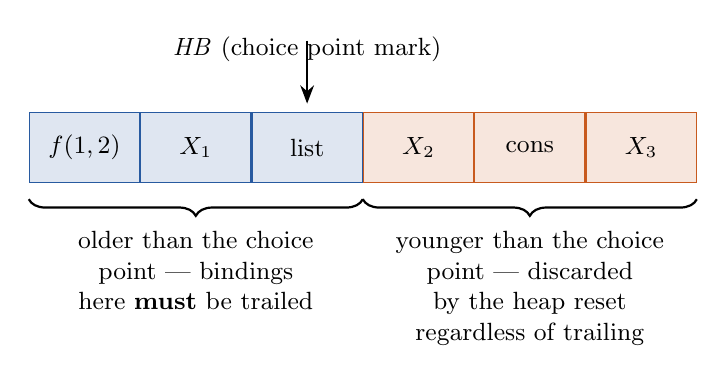
\begin{tikzpicture}[
  cell/.style={draw, minimum width=1.4cm, minimum height=0.9cm, font=\small},
  oldcell/.style={cell, fill=oldnode!15, draw=oldnode},
  youngcell/.style={cell, fill=youngnode!15, draw=youngnode},
]
  % heap as a row of cells, growing to the right
  \node[oldcell] (h0) {$f(1,2)$};
  \node[oldcell, right=0 of h0] (h1) {$X_1$};
  \node[oldcell, right=0 of h1] (h2) {list};
  \node[youngcell, right=0 of h2] (h3) {$X_2$};
  \node[youngcell, right=0 of h3] (h4) {cons};
  \node[youngcell, right=0 of h4] (h5) {$X_3$};

  \draw[-{Stealth}, thick] ($(h2.north)+(0,0.9)$) -- ($(h2.north)+(0,0.1)$)
    node[midway, above, font=\small] {$\mathit{HB}$ (choice point mark)};

  \draw[decorate, decoration={brace, amplitude=6pt, mirror}, thick]
    ($(h0.south west)+(0,-0.2)$) -- ($(h2.south east)+(0,-0.2)$)
    node[midway, below=8pt, font=\small, text width=3.6cm, align=center]
      {older than the choice point --- bindings here \textbf{must} be trailed};
  \draw[decorate, decoration={brace, amplitude=6pt, mirror}, thick]
    ($(h3.south west)+(0,-0.2)$) -- ($(h5.south east)+(0,-0.2)$)
    node[midway, below=8pt, font=\small, text width=3.6cm, align=center]
      {younger than the choice point --- discarded by the heap reset regardless of trailing};
\end{tikzpicture}
\caption{The WAM heap at the moment of a choice point (mark $\mathit{HB}$)
and after some further, forward computation. Bindings to the blue
(pre-existing) cells need trail entries; bindings to the orange (freshly
allocated since the choice point) cells don't, because backtracking's own
heap-pointer reset discards them unconditionally.}
\label{fig:wam-heap}
\end{figure}

This check is sound in the WAM specifically because of the \emph{binding
convention}: unification always binds the \emph{younger} variable to the
\emph{older} term, never the reverse. If an old, surviving variable were
ever bound to point at a young, about-to-be-discarded cell, resetting the
heap past that young cell would leave the old variable dangling. The WAM's
binding-order rule exists specifically to make the age-based trail
shortcut sound.

\section{How Rice implements the analogous check}

Rice has no bump-allocated heap and no single global ``pointer reset''
operation --- nodes are individually heap-allocated (\texttt{alloc()},
\texttt{runtime/memory.h}) and never explicitly freed on backtrack. So
there is no address-comparison-against-a-heap-mark to borrow directly.
Instead, \btomd's \#5 adapts the same idea
using an explicit logical clock:

\begin{itemize}
  \item A global counter, \texttt{current\_epoch} (\texttt{runtime.c}),
    starts at 0 and is incremented once per choice point created ---
    every call to \texttt{choose()} (resolving a live \texttt{?}) or
    \texttt{push\_choice()} (resolving a free variable against one of
    several constructors).
  \item Every node, at the moment it is \emph{freshly allocated}, is
    stamped with the counter's current value: a new \texttt{epoch} field
    on \texttt{Node} (\texttt{node.h}, compiled in only under the flag).
    This needed finding \emph{every} node-allocating site, not just the
    obvious ones: \texttt{Rice.Codegen.C.ToH}'s generated
    \texttt{make\_X}/\texttt{make\_X\_free} constructor/free-variable
    templates, and \texttt{runtime.h}/\texttt{runtime.c}'s own
    hand-written \texttt{make\_forward}, \texttt{make\_choice},
    \texttt{free\_var}, \texttt{make\_apply\{1,2,3\}}, \texttt{copy()},
    and \texttt{set\_copy\_free()}.
  \item \texttt{push\_node} --- the function that decides whether a node
    about to be mutated needs a trail entry at all (already gated by \#1
    on \texttt{nondet}) --- adds the age check on top:
\end{itemize}

\begin{lstlisting}[language=C]
static inline void push_node(union field root, bool nondet)
{
    root.n->nondet = nondet;
#if OPT_EPOCH_TRAIL
    if(nondet && root.n->epoch < current_epoch)
#else
    if(nondet)
#endif
    {
        stack_push(bt_stack, root, copy(root), false);
    }
}
\end{lstlisting}

\texttt{root.n->epoch < current\_epoch} is Rice's version of ``$a <
\mathit{HB}$'': the node was allocated before the currently-active choice
point, so it might be read again after backtracking and must be trailed.
When the node's epoch is not older than the active choice
($\mathtt{epoch} \ge \mathtt{current\_epoch}$), it was allocated \emph{as
part of} exploring the current alternative, and \#5's claim is the same
as the WAM's: nothing outside this exploration could hold a valid
reference to it, so skip the trail push.

The stack-frame bookkeeping needed to make this correct across
backtracking is unconditional, not compiled out when the flag is off, so
that \texttt{choose()}/\texttt{push\_choice()} are the only two places
that need to know the flag exists for the stack half of this at all:
\texttt{FieldPair} (\texttt{stack.h}) carries an \texttt{epoch} field,
snapshotted on every \texttt{stack\_push} and restored on every
\texttt{pop}/\texttt{pop\_to} (\texttt{stack.c}), regardless of
\texttt{OPT\_\allowbreak EPOCH\_\allowbreak TRAIL}.

\section{Why it doesn't fire}
\label{sec:why-not}

Measured directly (\texttt{tests/bench.sh}, \texttt{STATUS.md}'s
2026-09-12 entry): across all ten \texttt{SLOW}-tagged benchmarks,
\texttt{OPT\_\allowbreak EPOCH\_\allowbreak TRAIL} produces \emph{bit-for-bit identical} total
allocation counts to the shipped defaults, and is consistently 3--15\%
\emph{slower} (pure bookkeeping overhead, no payoff). A microbenchmark
built specifically to hit \#5's precondition --- one long-lived outer
choice, with 5000 recursive steps underneath it each reading a second,
already-resolved choice --- \emph{also} shows zero difference. This isn't
several unlucky test programs; there's a structural reason.

\subsection{\texttt{undo()} restores a whole node, pointers included}

\begin{lstlisting}[language=C]
bool undo(int cutoff)
{
    ...
    do
    {
        frame = pop(bt_stack);
        if(frame->lhs.n != NULL)
        {
            memcpy(frame->lhs.n, frame->rhs.n, sizeof(Node));
        }
    } while(!frame->choice && size(bt_stack) > cutoff);
    ...
}
\end{lstlisting}

Restoring a trailed node's saved snapshot overwrites \emph{all} of its
fields, including whatever child pointers it held. So restoring \emph{one}
mutated ancestor automatically discards access to everything that was
built \emph{underneath} it during the abandoned exploration --- regardless
of whether any of those descendant nodes were individually trailed at all.
The only node that ever needs its own trail entry, for any given piece of
nested computation, is the \emph{outermost} node that is both mutated and
directly touches nondeterminism.

\subsection{That outermost node is always older than what's nested inside it}

This is the point that closes off \#5's opportunity almost entirely: to
even \emph{reach} a choice nested three function calls deep, something
has to already exist and already be under evaluation to make those three
calls. That something's own reduction is what the case-dispatch or
apply-resolution machinery marks \texttt{nondet = true} on, and it was, by
definition, allocated \emph{before} the nested choice it eventually
reaches. It can never be ``young'' relative to a choice nested inside its
own evaluation --- the containment relationship forces the age ordering
the other way around. For \#5 to find anything to skip, a node would need
to be simultaneously (a) directly, independently nondet-tainted by
touching some choice/free variable in its \emph{own} right, and (b)
younger than a \emph{different}, already-active outer choice --- i.e.\
genuinely separate, parallel nondeterminism nested inside an active
choice's scope, not merely ``deep recursion under a choice'', no matter
how deep.

\subsection{Graphs}

Figure~\ref{fig:rice-before} shows the shape of the microbenchmark's graph
while evaluating one branch of the outer choice: an old, top-level
expression node \texttt{M} (older than the active choice, because it had
to already exist and be forced to reach it) dominates a long chain of
freshly-built application nodes from unrolling \texttt{loop}. Every node
in that chain is young relative to the active choice, but \emph{none of
them is individually nondet} --- reading the resolved value of \texttt{f}
through an ordinary argument doesn't propagate a taint onto the node built
from it; only \texttt{f}'s own node (marked directly by \texttt{choose()})
and \texttt{M} (marked because \emph{its} own reduction dispatches
directly on a live choice) are ever candidates for the trail at all.

\begin{figure}[htb]
\centering
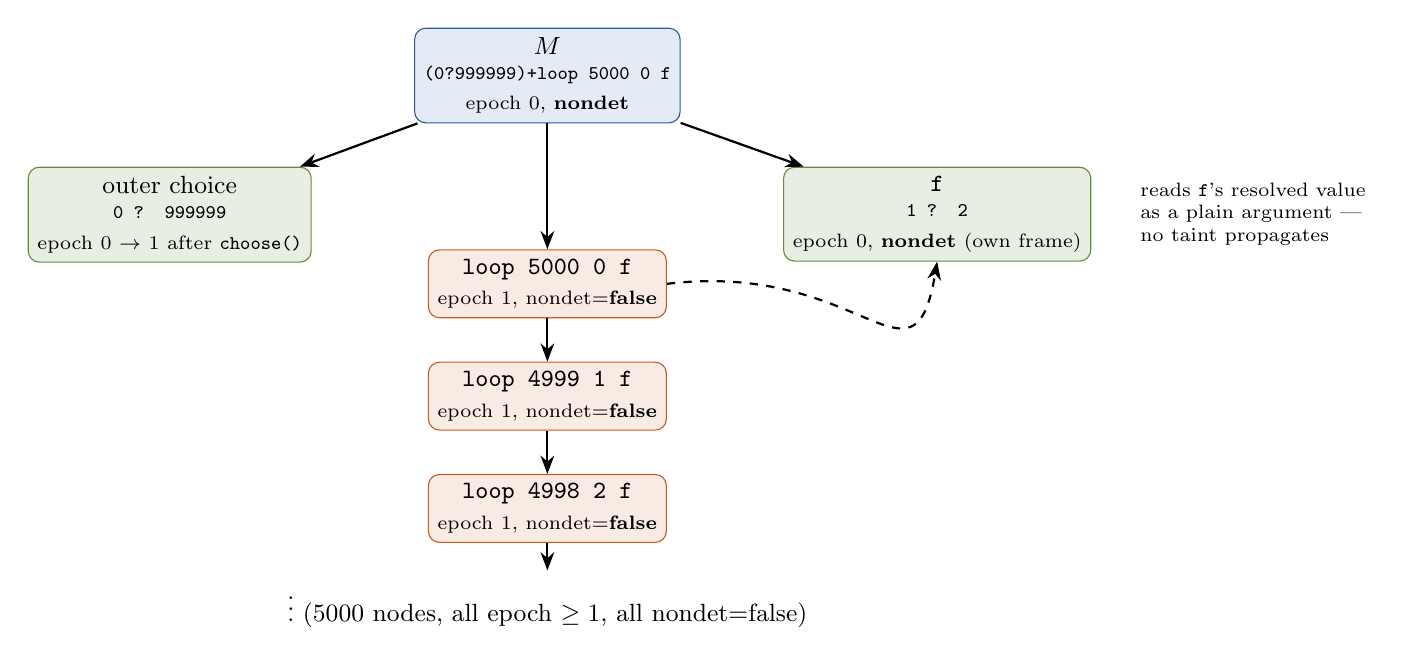
\begin{tikzpicture}[
  node distance=0.55cm and 1.3cm,
  oldbox/.style={draw=oldnode, fill=oldnode!12, rounded corners, minimum width=2.6cm, minimum height=0.9cm, font=\small, align=center},
  youngbox/.style={draw=youngnode, fill=youngnode!12, rounded corners, minimum width=2.2cm, minimum height=0.8cm, font=\small, align=center},
  choicebox/.style={draw=choicenode, fill=choicenode!15, rounded corners, minimum width=2.2cm, minimum height=0.8cm, font=\small, align=center},
  note/.style={font=\scriptsize, text width=3.1cm, align=left},
  arr/.style={-{Stealth}, thick},
]
  \node[oldbox] (M) {$M$\\[-2pt]\scriptsize \texttt{(0?999999)+loop\ 5000\ 0\ f}\\ \scriptsize epoch 0, \textbf{nondet}};
  \node[choicebox, below left=of M] (outer) {outer choice\\[-2pt]\scriptsize \texttt{0 ? 999999}\\ \scriptsize epoch 0 $\to$ 1 after \texttt{choose()}};
  \node[choicebox, below right=of M] (f) {\texttt{f}\\[-2pt]\scriptsize \texttt{1 ? 2}\\ \scriptsize epoch 0, \textbf{nondet} (own frame)};
  \node[note, right=0.5cm of f] (fnote) {reads \texttt{f}'s resolved value as a plain argument --- no taint propagates};

  \node[youngbox, below=1.6cm of M] (l1) {\texttt{loop 5000 0 f}\\ \scriptsize epoch 1, nondet=\textbf{false}};
  \node[youngbox, below=of l1] (l2) {\texttt{loop 4999 1 f}\\ \scriptsize epoch 1, nondet=\textbf{false}};
  \node[youngbox, below=of l2] (l3) {\texttt{loop 4998 2 f}\\ \scriptsize epoch 1, nondet=\textbf{false}};
  \node[below=0.35cm of l3, font=\small] (dots) {$\vdots$ (5000 nodes, all epoch $\ge 1$, all nondet=false)};

  \draw[arr] (M) -- (outer);
  \draw[arr] (M) -- (f);
  \draw[arr] (M) -- (l1);
  \draw[arr] (l1) -- (l2);
  \draw[arr] (l2) -- (l3);
  \draw[arr] (l3) -- (dots);
  \draw[arr, dashed] (l1.east) .. controls +(2.5,0.3) and +(-0.3,-1.8) .. (f.south);
\end{tikzpicture}
\caption{The microbenchmark's graph while exploring one branch. \texttt{M}
(blue) is the one node whose own reduction directly dispatches on a live
choice, so it is the one node \#1 marks \texttt{nondet} and pushes to the
trail. The entire \texttt{loop} chain (orange) is young relative to the
active choice, but every node in it has \texttt{nondet=false} --- \#1
already excludes all of them from the trail, so \#5's age check never even
gets a candidate to filter.}
\label{fig:rice-before}
\end{figure}

Figure~\ref{fig:rice-after} shows what \texttt{undo()} does when
backtracking reaches the outer choice: popping \texttt{M}'s trail frame
overwrites \texttt{M}'s fields with its saved, pre-evaluation snapshot ---
including the pointer that used to lead into the \texttt{loop} chain. That
whole chain becomes unreachable in one step, independent of whether any
node in it was ever individually trailed.

\begin{figure}[htb]
\centering
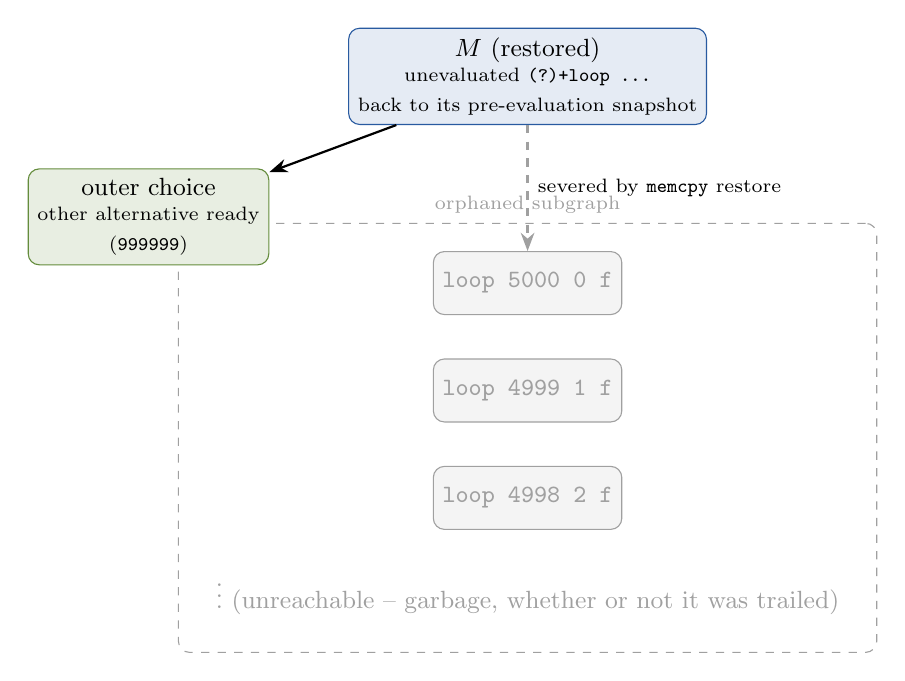
\begin{tikzpicture}[
  node distance=0.55cm and 1.0cm,
  oldbox/.style={draw=oldnode, fill=oldnode!12, rounded corners, minimum width=2.6cm, minimum height=0.9cm, font=\small, align=center},
  deadbox/.style={draw=deadnode, fill=deadnode!12, rounded corners, minimum width=2.2cm, minimum height=0.8cm, font=\small, align=center, text=deadnode},
  choicebox/.style={draw=choicenode, fill=choicenode!15, rounded corners, minimum width=2.2cm, minimum height=0.8cm, font=\small, align=center},
  arr/.style={-{Stealth}, thick},
  deadarr/.style={-{Stealth}, thick, dashed, draw=deadnode},
]
  \node[oldbox] (M) {$M$ (restored)\\[-2pt]\scriptsize unevaluated \texttt{(?)+loop\ ...}\\ \scriptsize back to its pre-evaluation snapshot};
  \node[choicebox, below left=of M] (outer) {outer choice\\[-2pt]\scriptsize other alternative ready\\ \scriptsize (\texttt{999999})};

  \node[deadbox, below=1.6cm of M] (l1) {\texttt{loop 5000 0 f}};
  \node[deadbox, below=of l1] (l2) {\texttt{loop 4999 1 f}};
  \node[deadbox, below=of l2] (l3) {\texttt{loop 4998 2 f}};
  \node[below=0.35cm of l3, font=\small, text=deadnode] (dots) {$\vdots$ (unreachable -- garbage, whether or not it was trailed)};

  \begin{scope}[on background layer]
    \node[fit=(l1)(l2)(l3)(dots), draw=deadnode, dashed, rounded corners, inner sep=10pt, label={[deadnode]above:\scriptsize orphaned subgraph}] {};
  \end{scope}

  \draw[arr] (M) -- (outer);
  \draw[deadarr] (M.south) -- (l1.north)
    node[midway, right, font=\scriptsize] {severed by \texttt{memcpy} restore};
\end{tikzpicture}
\caption{After \texttt{undo()} pops \texttt{M}'s frame and backtracks to
the outer choice: \texttt{M} is restored to its exact pre-evaluation
content, including its pointer fields, which no longer lead into the
\texttt{loop} chain at all. Whatever was built during this exploration is
orphaned in one step. Nothing needed to check \texttt{loop}'s nodes'
individual ages for this to be correct -- they were never going to be
read again either way.}
\label{fig:rice-after}
\end{figure}

\subsection{The contrast with Prolog, restated}

In the WAM, \emph{every} unification --- deterministic or not --- goes
through the same bind-and-maybe-trail path, so an age filter is cutting a
large, otherwise-undifferentiated population down to size. Rice's \#1
already removes purely deterministic reduction from the trail machinery
entirely (Figure~\ref{fig:rice-before}'s whole \texttt{loop} chain is an
example: 5000 nodes, zero trail candidates, with or without \#5). What's
left over after \#1 is a small population that is, by the containment
argument above, already dominated by nodes old enough to need trailing
regardless of \#5's check. Rice gets most of what the WAM's optimization
buys Prolog for free, via sharing and \#1, rather than needing the
explicit age check to buy a second, separate slice of it.

\section{Status}

Kept in the codebase, \texttt{OPT\_\allowbreak EPOCH\_\allowbreak TRAIL} defaulting off, rather
than removed: the goal per \btomd is
eventually reporting how much \emph{each} backtracking optimization
contributes empirically (\texttt{tests/bench.sh}), and a documented,
measured ``this one doesn't help, here is why'' is itself a useful data
point for that report, not dead weight to delete. If a workload is ever
found with genuinely separate, nested nondeterminism inside an
already-active choice's scope --- something other than the
generate-then-deterministically-verify shape common to
\texttt{old\_rice/\allowbreak benchmarks/} --- it would be a natural candidate to
re-test \#5 against.

\end{document}
